\chapter{Chiffrement RSA}

\section{Écrire un programme d'exponentiation rapide}

L'exponentiation rapide est une méthode permettant de calculer rapidement des grandes puissances de nombre. En effet, pour calculer de manière naïve $n^p$ avec $p$ très grand, c'est-à-dire en multipliant $n$ par lui-même $p$ fois, est très peu efficace.

\definecolor{lightgreen}{rgb}{0.56, 0.93, 0.56}


\begin{tcolorbox}[
    enhanced,
    attach boxed title to top left={xshift=6mm,yshift=-3mm},
    colback=lightgreen!20,
    colframe=lightgreen,
    colbacktitle=lightgreen,
    title=Algorithme naïf pour calculer $n^p$,
    fonttitle=\bfseries\color{black},
    boxed title style={size=small,colframe=lightgreen,sharp corners},
    sharp corners,
]
\begin{minted}{python}

# Algorithme naif
def basic_pow(n, p):
    res = 1
    for i in range(p):
        res *= n
    return res
\end{minted}
\end{tcolorbox}

Cependant, on regarde que si l'on écrit p en binaire ($p = \sum_{i \leq d}{a_i 2^i}$ avec $a_i \in \{0,1\}$), on peut réécrire $n^p$ comme suit :

$n_p = n^{a_0} (n^2)^{a_1} (n^{2^2})^{a_2} ... (n^{2^d})^{a_d}$. \\

\begin{tcolorbox}[
    enhanced,
    attach boxed title to top left={xshift=6mm,yshift=-3mm},
    colback=lightgreen!20,
    colframe=lightgreen,
    colbacktitle=lightgreen,
    title=Algorithme d'exponentiation rapide pour calculer $n^p$,
    fonttitle=\bfseries\color{black},
    boxed title style={size=small,colframe=lightgreen,sharp corners},
    sharp corners,
]    
    \begin{minted}{python}
# Algorithme d'exponentiation rapide
def fast_pow(n, p):
    res = 1
    # On divise consecutivement p par 2 jusqu'a ce que p soit nul
    while p > 0:
        # Si p est impair, on multiplie le resultat par n
        if p % 2 == 1:
            res *= n
        # On divise p par 2 et on multiplie n par lui-meme
        n *= n
        p //= 2
    return res
    \end{minted}
\end{tcolorbox}

Sur la figure \ref{fig:perf_exp_rapide}, on peut voir la différence de performance entre l'algorithme naïf (avec des multiplications successives) et l'algorithme d'exponentiation
binaire. Pour 10 itérations de $2^{1000000}$, l'algorithme naïf prend 168.49 secondes alors que l'algorithme d'exponentiation binaire prend 0.04 secondes. \\

\begin{figure}[H]
\centering
    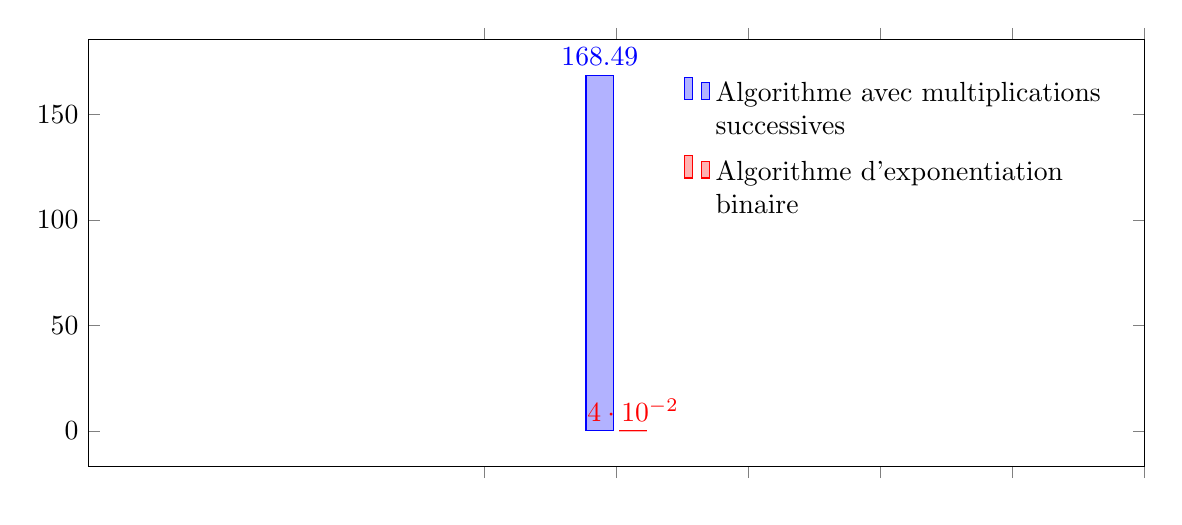
\begin{tikzpicture}
    
        \begin{axis} [
            ybar,
            nodes near coords,
            width=15cm,
            height=7cm,
            xticklabel=\empty,
            legend style={
                draw=none,
                text width=5cm,
                minimum height=1.0cm,
            }
        ]
        \addplot coordinates {
            (1,168.49)
        };
        \addplot coordinates {
            (1,0.04)
        };
        \legend {Algorithme avec multiplications successives, Algorithme d'exponentiation binaire};
        \end{axis}

    \end{tikzpicture}
\caption{Comparaison des performances des 2 algorithmes pour 10 itérations avec $2^{1000000}$} \label{fig:perf_exp_rapide}
\end{figure}

Pour les petits exposants, Python utilise l'exponentiation binaire\footnote{https://stackoverflow.com/questions/9434183/whats-the-fastest-algorithm-to-perform-exponentiation}.

\section{Écrire un programme de calcul des coefficients de Bézout}

On cherche à trouver $u$ et $v$ tels que $au + bv = pgcd(a,b)$. Pour cela, on utilise l'algorithme d'Euclide étendu. L'algorithme ci-dessous retourne $u$ et $v$ tels que $au + bv = pgcd(a,b)$ et $r = pgcd(a,b)$. \\

\begin{tcolorbox}[
    enhanced,
    attach boxed title to top left={xshift=6mm,yshift=-3mm},
    colback=lightgreen!20,
    colframe=lightgreen,
    colbacktitle=lightgreen,
    title=Calcul des coefficients de Bézout,
    fonttitle=\bfseries\color{black},
    boxed title style={size=small,colframe=lightgreen,sharp corners},
    sharp corners,
]    
    \begin{minted}{python}
def bezout_coeff(a, b):
    # Algorithme d'Euclide étendue
    r, u, v, r_prime, u_prime, v_prime = a, 1, 0, b, 0, 1
    while r_prime != 0:
        q = r // r_prime
        r = r_prime
        u = u_prime
        v = v_prime
        r_prime = r - q * r_prime
        u_prime = u - q * u_prime
        v_prime = v - q * v_prime
    return u, v, r

print(bezout_coeff(123, 456)) # (-63, 17, 3)
    \end{minted}
\end{tcolorbox}

\section{Écrire un programme de chiffrement RSA}

On doit tout d'abord commencer par choisir deux nombres $p$ et $q$ qui sont premiers et distincts. On a donc créé une fonction pour vérifier si un nombre est premier et une fonction pour en générer. Pour tester si un nombre est premier, on teste tous les nombres de 2 à $\sqrt{n}$ (on peut s'arrêter à $\sqrt{n}$ car si $n$ n'est pas premier, il existe un diviseur $d$ de $n$ tel que $d \leq \sqrt{n}$). Pour générer un nombre premier, on génère un nombre aléatoire entre 100 et 1000 et on teste s'il est premier. Si ce n'est pas le cas, on en génère un autre. \\

\begin{tcolorbox}[
    enhanced,
    attach boxed title to top left={xshift=6mm,yshift=-3mm},
    colback=lightgreen!20,
    colframe=lightgreen,
    colbacktitle=lightgreen,
    title=Test de primalité et génération de nombres premiers,
    fonttitle=\bfseries\color{black},
    boxed title style={size=small,colframe=lightgreen,sharp corners},
    sharp corners,
]    
    \begin{minted}{python}
import math

# Fonction qui vérifie si un nombre est premier
def is_prime(n):
    if n < 2:
        return False
    for i in range(2, int(math.sqrt(n)) + 1, 2):
        if n % i == 0:
            return False
    return True

# Génération de nombres premiers
def generate_prime():
    p = random.randint(100, 1000)
    while not is_prime(p):
        p = random.randint(100, 1000)
    return p

p = generate_prime()
q = generate_prime()

# On vérifie que p et q sont distincts
while p == q:
    q = generate_prime()

    \end{minted}
\end{tcolorbox}

Ensuite, on peut générer la clé publique en calculant $n = pq$ et $\phi(n) = (p-1)(q-1)$. On choisit ensuite un nombre $e$ tel que $1 < e < \phi(n)$ et $pgcd(e, \phi(n)) = 1$. Grâce au théorème de Bézout, on trouve $d \times e \equiv 1 \mod \phi(n)$ (qui est utilisé pour la clé privée). \\

\begin{tcolorbox}[
    enhanced,
    attach boxed title to top left={xshift=6mm,yshift=-3mm},
    colback=lightgreen!20,
    colframe=lightgreen,
    colbacktitle=lightgreen,
    title=Génération de la clé publique et privée,
    fonttitle=\bfseries\color{black},
    boxed title style={size=small,colframe=lightgreen,sharp corners},
    sharp corners,
]    
    \begin{minted}{python}
def generate_keys(p, q):
    # Vérification que p et q sont premiers
    assert(is_prime(p))
    assert(is_prime(q))
    assert(p != q)

    n = p * q
    phi = (p - 1) * (q - 1)

    # On choisit un entier e tel pgcd(e, phi) = 1
    e = random.randint(2, phi - 1)
    while pgcd(e, phi) != 1:
        e = random.randint(2, phi - 1)

    # On calcule d tel que e * d = 1 (mod phi)
    d = bezout_coeff(e, phi)[0]
    if d < 0:
        d += phi

    # On retourne la clé publique et la clé privée
    return (e, n), (d, n)
    \end{minted}
\end{tcolorbox}

Nous créons ensuite les fonctions pour chiffrer et déchiffrer un message. Pour chiffrer un message, on utilise la clé publique $(e, n)$ et on calcule $c = m^e \mod n$. Pour déchiffrer un message, on utilise la clé privée $(d, n)$ et on calcule $m = c^d \mod n$. \\

\begin{tcolorbox}[
    enhanced,
    attach boxed title to top left={xshift=6mm,yshift=-3mm},
    colback=lightgreen!20,
    colframe=lightgreen,
    colbacktitle=lightgreen,
    title=Chiffrement et déchiffrement d'un message,
    fonttitle=\bfseries\color{black},
    boxed title style={size=small,colframe=lightgreen,sharp corners},
    sharp corners,
]    
    \begin{minted}{python}
# Chiffrement
def encrypt(public_key, message):
    e, n = public_key
    return fast_pow(message, e) % n

# Déchiffrement
def decrypt(private_key, message):
    d, n = private_key
    return fast_pow(message, d) % n
    \end{minted}
\end{tcolorbox}

Enfin, on utilise notre programme en commençant par générer $p$ et $q$ premiers et distincts. On génère ensuite les clés publique et privée. On peut ensuite chiffrer et déchiffrer un message. On s'assure que le message déchiffré est bien égal au message initial. \\

\begin{tcolorbox}[
    enhanced,
    attach boxed title to top left={xshift=6mm,yshift=-3mm},
    colback=lightgreen!20,
    colframe=lightgreen,
    colbacktitle=lightgreen,
    title=Test de notre programme de chiffrement RSA,
    fonttitle=\bfseries\color{black},
    boxed title style={size=small,colframe=lightgreen,sharp corners},
    sharp corners,
]    
    \begin{minted}{python}
# Test de chiffrement et déchiffrement avec des nombres aléatoires
p = 5
q = 17

while p == q:
    q = generate_prime()


message = 10
public_key, private_key = generate_keys(p, q)

encrypted_message = encrypt(public_key, message)
decrypted_message = decrypt(private_key, encrypted_message)

assert(message == decrypted_message)
    \end{minted}
\end{tcolorbox}